\chapter{Programska potpora za korisničko sučelje}

Za bolje korisničko iskustvo kreirano je grafičko korisničko sučelje (engl. \textit{Graphic User Interface} - GUI) koje se izvodi na korisničkom računalu. U GUI aplikaciji moguće je pokrenuti snimanje novog audiozapisa te grafički prikazati obradu signala postojećeg zvuka na računalu. 

\section{Razvojni alat PyQt} 
Aplikacija je izrađena korištenjem razvojnog alata PyQt temeljenog na programskom
jeziku Python i pripadnih biblioteka za razvoj grafičkih korisničkih sučelja. PyQt je priključak (engl. \textit{plug-in}) za Python - mostna biblioteka između Pythona i razvojnog alata Qt, koji podržava programski jezik C++. Korištena je inačica \textit{PyQt5}, koja je kompatibilna s Python 3 verzijom.

Osnova \textit{Qt} aplikacija je objektni model koji, koristeći sustav \textit{Meta Object} i klasu \textit{QObject}, proširuje funkcionalnost standardnog programskog jezika C++ i time omogućuje razvoj grafičkih korisničkih sučelja. \textit{PyQt} omata funkcionalnosti \textit{Qt} radnog okvira te ih prilagođava programskom jeziku Python, odnosno kombinira kompleksnost alata za razvoj grafičkog sučelja i jednostavnost programskog jezika.

Osnovna klasa je \textit{QObject} koja pruža sljedeće funkcionalnosti:
\begin{itemize}
	\item definiranje objekata jedinstvenim imenom,
	\item hijerarhijska organizacija objekata,
	\item komunikacija između objekata, 
	\item upravljanje događajima.
\end{itemize}

Komunikacija između \textit{Qt} objekata odvija se mehanizmom signala i utora (engl. \textit{signals and slots}). Signal se emitira pri promjeni stanja objekta, primjerice pritiskom na gumb unutar korisničkog sučelja. Pri emisiji signala poziva se funkcija utora s kojom je taj signal povezan te se obrađuje događaj koji je izazvao emisiju. 

Stvaranje i uređivanje grafičkih elemenata (engl. \textit{widgets}) omogućeno je klasom \textit{QWidget}. Grafički elementi organizirani su hijerarhijski, pri čemu je glavni prozor "roditelj" ostalih elemenata. 

\section{Implementacija korisničkog sučelja}

Pri pokretanju aplikacije, u glavnom prozoru prikazuje se izbornik s gumbima \textit{Record} i \textit{Analyse Audio}. \textit{Record} gumb vodi na sučelje za podešavanje parametara snimanja, dok \textit{Analyse Audio} otvara meni za odabir audio datoteke za analizu.

\begin{figure}[ht]
	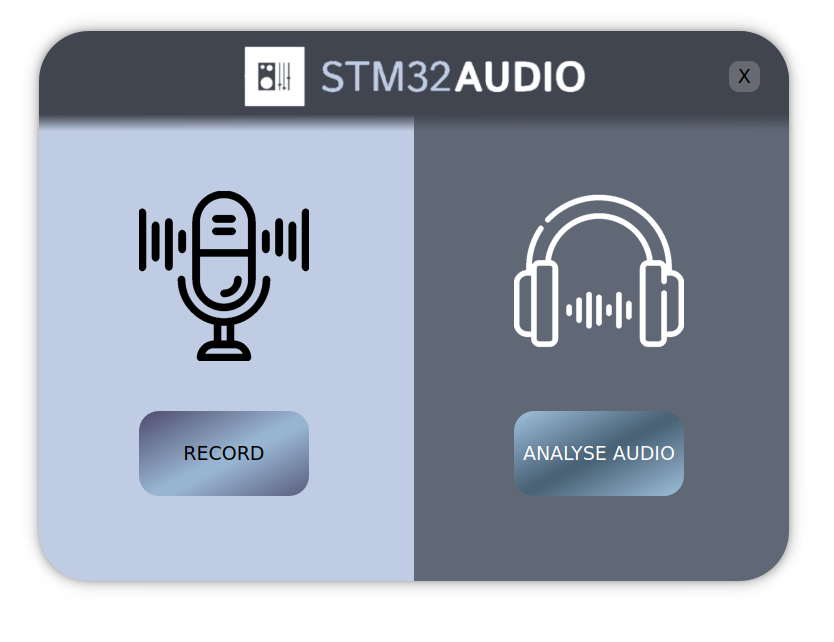
\includegraphics[width=\linewidth]{imgs/intro_form}
	\caption{Uvodni izbornik}
	\label{fig:intro_form}
\end{figure}

Nakon otvaranja audio datoteke, vrši se obrada zvučnog signala. Audio biblioteka \textit{SoundFile} koristi se za učitavanje audio datoteke te, pozivom 
\begin{lstlisting}
	sf.read(file_path)
\end{lstlisting}	
dobivaju se matrica amplituda i frekvencija uzorkovanja. Dobivena matrica reprezentacija je audio signala u vremenskoj domeni, odnosno prikazuje glasnoću (amplitudu) zvuka dok se mijenja u vremenu. Amplituda jednaka nuli označava tišinu.

Za analizu odnosa amplitude i frekvencije signala potrebno transformirati signal u frekvencijsku domenu kako bi se prikazalo koje frekvencije se nalaze u signalu. Fourierovom transformacijom signal se dekomponira u odgovarajuće frekvencije. \textit{Scipy} biblioteka sadrži ugrađenu funkciju za brzu Fourierovu transformaciju.

\lstinputlisting[language=Python, firstline=53, lastline=56, caption=Fourierova transformacija]{./../BlueSTSDK_Python/blue_st_examples/analysis.py}


Dobivene matrice iscrtavaju se grafički pomoću biblioteke \textit{matplotlib}. Ograničen je prikaz frekvencija na 2000 Hz...

\begin{figure}[ht]
	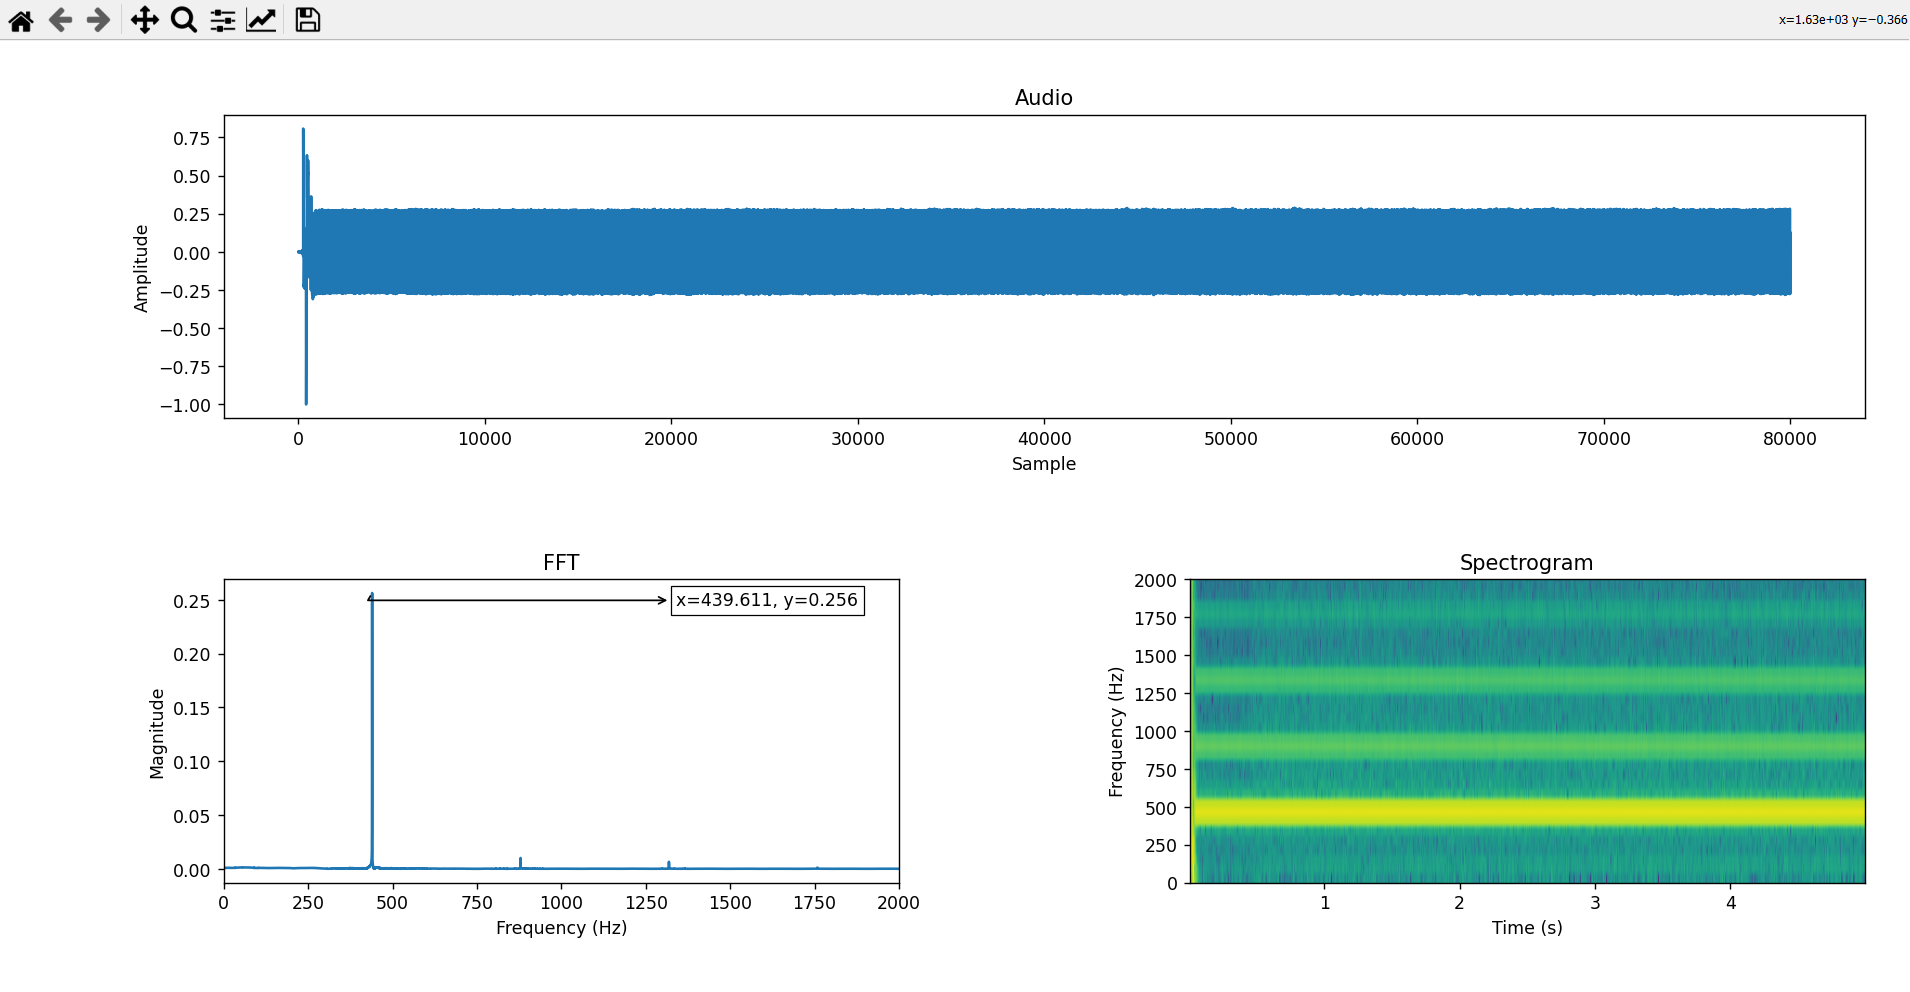
\includegraphics[width=\linewidth]{imgs/analyse_example}
	\caption{Primjer prikaza analize audiozapisa}
	\label{fig:analyse_example}
\end{figure}

Ovdje će biti tekst koji govori o odabiru parametara.

\begin{figure}[ht]
	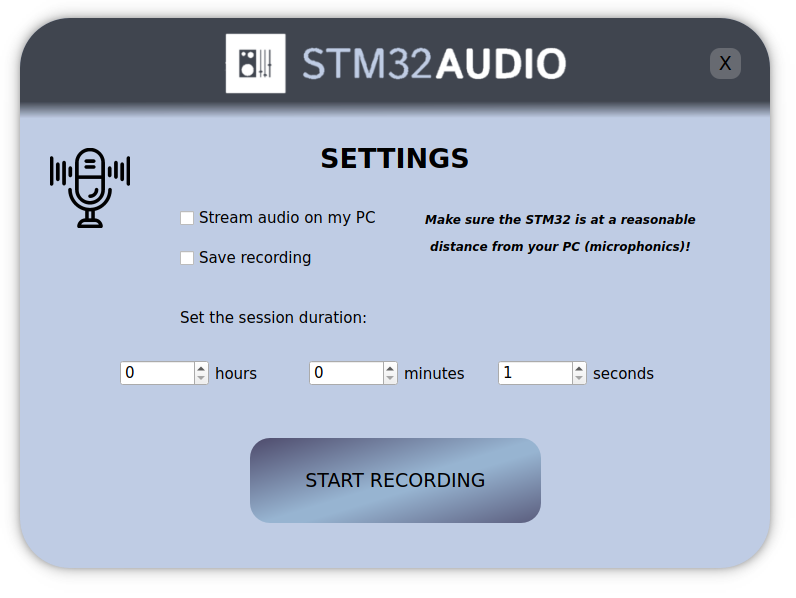
\includegraphics[width=\linewidth]{imgs/params_form}
	\caption{Sučelje za podešavanje parametara}
	\label{fig:params_form}
\end{figure}

%%
%mini slikice%
\begin{figure}[ht]
	\begin{minipage}[t]{0.4\textwidth}
		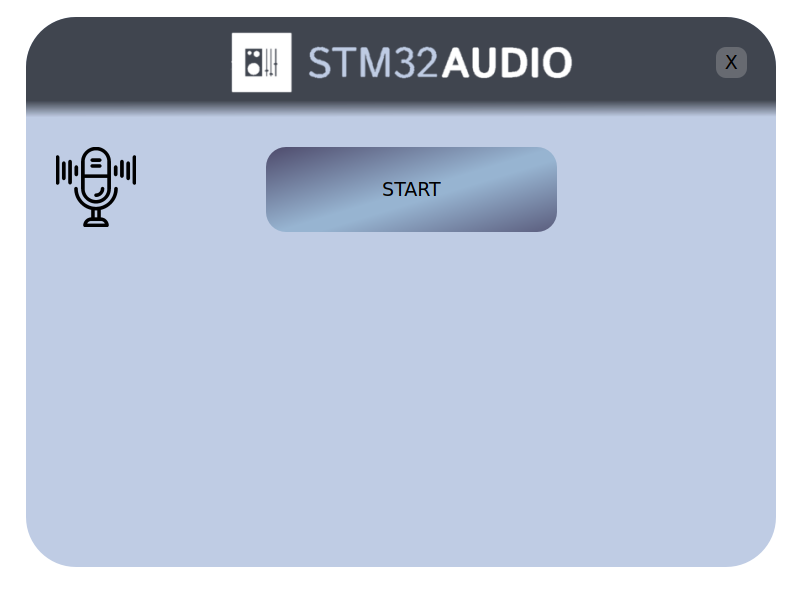
\includegraphics[width=\linewidth]{imgs/recording_form}
		\caption{Prije pokretanja snimanja}
		\label{fig:recording_form}
	\end{minipage}
	\hspace*{\fill}
	\begin{minipage}[t]{0.4\textwidth}
		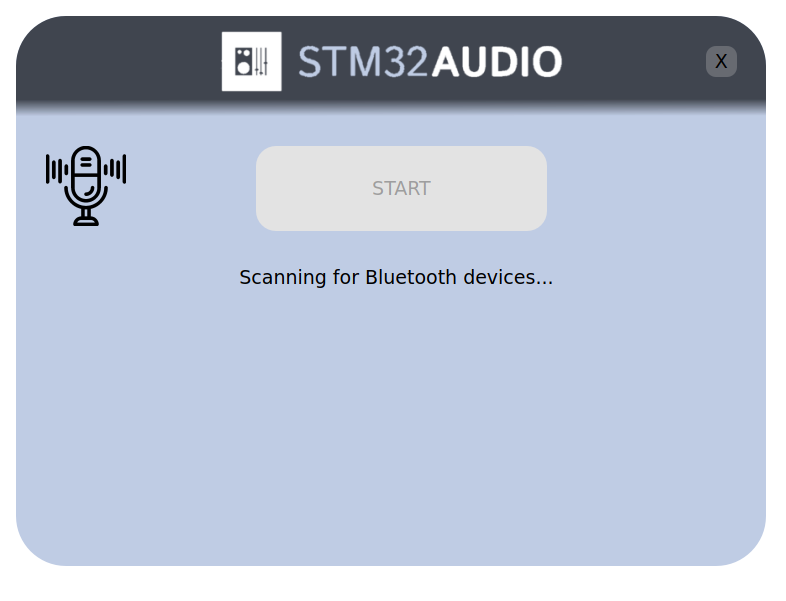
\includegraphics[width=\linewidth]{imgs/recording_form_2}
		\caption{Skeniranje uređaja}
		\label{fig:recording_form_2}
	\end{minipage}
\end{figure}

\begin{figure}[ht]
	\begin{minipage}[t]{0.4\textwidth}
	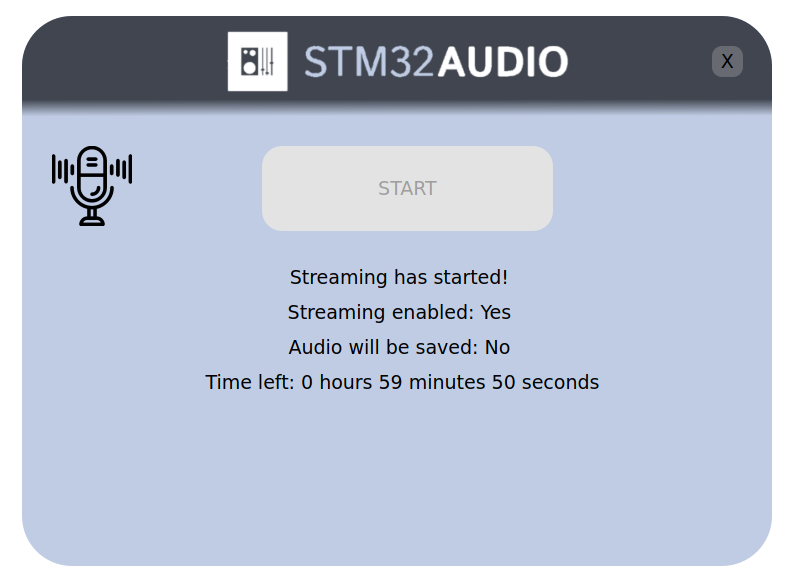
\includegraphics[width=\linewidth]{imgs/recording_form_3}
	\caption{Snimanje zvuka}
	\label{fig:recording_form_3}
	\end{minipage}
	\hspace*{\fill}
	\begin{minipage}[t]{0.4\textwidth}
		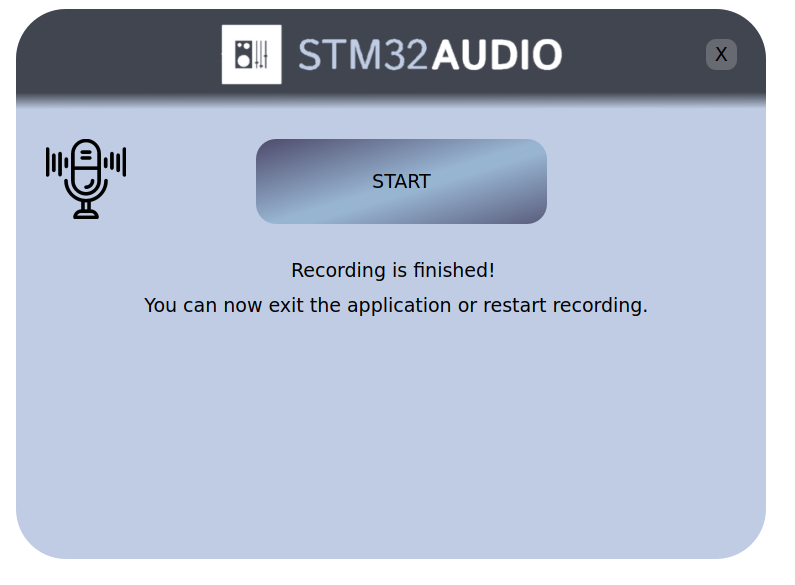
\includegraphics[width=\linewidth]{imgs/recording_form_4}
		\caption{Završetak snimanja}
		\label{fig:recording_form_4}
	\end{minipage}
\end{figure}
%end mini slikice%
%%

\eject